\begin{python0}
from solutions import *; clear()
\end{python0}
\sectionthree{Variables with the same name}

Pay attention!!! This is something new!!!

You can actually create variables with the same name ... provided they
are either declared in non-overlapping blocks or one is defined in an
inner block.

Here' s the case where names are created in \EMPHASIZE{disjoint blocks}:

\begin{consolethree}[escapeinside=||]
...

for (int i = 0; i < 10; ++i)
{   
     int x, y, z;
     ...
}

|\tikzmarknode{disjointnode}{for (int i = 0; i < 100; ++i)}\sidebox{disjointbox}{No problem! You won't get a re-declaration because the previous i is already destroyed!}||\DrawArrow{disjointbox}{disjointnode}|
{   
     ...
     int y;

}

... 
\end{consolethree}

Do you see why there won' t be conflicts or confusion to C++?

Here' s the case where two names are created in \EMPHASIZE{nested blocks}:
\sidenote
{
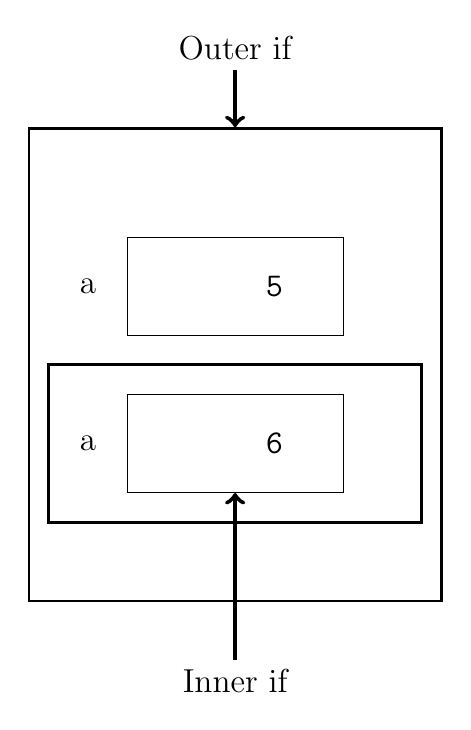
\begin{tikzpicture}
\node[draw, line width=1,text width=5cm, minimum height=6cm] (nestboxA) at (0,0) {};

\node[yshift=1cm,draw, line width=0.2,text width=2.5cm, minimum height=1.25cm] (nestboxB) at (nestboxA.center) {\large\texttt{\ \ \ \ \ \ \ \ \ \ \ \ \ \ 5}};

\node[yshift=-1cm,draw, line width=0.2,text width=2.5cm, minimum height=1.25cm] (nestboxC) at (nestboxA.center) {\large\texttt{\ \ \ \ \ \ \ \ \ \ \ \ \ \ 6}};

\node[draw, line width=1,text width=4.5cm, minimum height=2cm] (nestboxD) at (nestboxC.center) {};
\node[yshift=1cm] (nestouterif) at (nestboxA.north){\large{Outer if}};
\node[yshift=-1cm] (nestinnerif) at (nestboxA.south){\large{Inner if}};
\node[xshift=-5mm] (nestoutera) at (nestboxB.west) {\large{a}};
\node[xshift=-5mm] (nestinnera) at (nestboxC.west) {\large{a}};
\draw[ultra thick, ->] (nestouterif) to (nestboxA.north);
\draw[ultra thick, ->] (nestinnerif) to (nestboxC.south);
\end{tikzpicture}
}
\begin{console}
int x = 0, y = 0;
std::cin >> x >> y;

if (x == 0)
{    
     int a = 5;
     std::cout << a << std::endl;

     if (y == 1)
     {
          int a = 6;
          std::cout << a << std::endl;
     }
}
\end{console}

YIKES!!!

Note that the first print statement is not ambiguous. (Why?)

But what about the second? Which \texttt{a} is used in the second print statement???... go to next section to find out ...

WARNING: Although technically you can do the above (i.e. have two variables with the same name nest within blocks, it makes the code hard to read. Not only that, some languages do not allow this at all. Therefore you should \EMPHASIZE{AVOID DECLARING VARIABLES WITH THE SAME NAME IN NESTED BLOCKS}. The only \EMPHASIZE{exception} is a temporary (scratch) variable for instance like the counter variable of a \texttt{for}-loop

\begin{console}
for (int i = 0; i < 100; i++)
{    
     ...
     for (int i = -10; i < 10; i++)
     {    
          ...
     }
     ...
}
\end{console}

and only when the logic is easy to understand. But even then, you might still be shooting yourself in your foot later if you need to change the logic of your code.

